\section{Application}
\label{sub:examples}

A comparative study was conducted to analyze the impact of using real data on delivery simulation metrics across three different cases, while demonstrating the possibilities of our solution. The first case, a baseline scenario, represents synthetic bus lines and tasks. The second case represents a suburban environment, that is the area surronding bus line 705 that radiate from EPFL to the small villages in the direction of Morges, while the third case represents a city area, namely the Lausanne agglomeration. 

\subsection{Baseline case : synthetic bus lines and tasks}

For this case, we consider a rectangle of 70 x 80 space units. Two bus lines are set up, each with 12 bus stations equally spaced, their central parts making a square around the city center, while tasks are taken from the \href{https://www.sintef.no/projectweb/top/pdptw/100-customers/}{PDPTW dataset}. 50 tasks are considered for this case, altough 2 tasks have the same pickup and delivery point. Figure \ref{fig:synthetic_tasks} represents this case.

\addfigure[synthetic_tasks]{synthetic_tasks.png}{Our baseline case}

\subsection{Suburban case : Bus line 705}

Here, we took bus line 705 from EPFL to represent a suburban environment. This bus line links EPFL to the Lonay village, passing through the villages of Ecublens, Echandens, Denges and Préverenge. We defined the study area as a rectangle fitting every stop of the bus line with a margin of 500m on each side.
As can be seen on Figure \ref{fig:suburban_case}, the line makes a Z-shape in order to desserve most villages in the area. Altough this reduces the interest of the line for users, it could make it very usefull in our case, by desserving most customers and shops.

\begin{figure}
     \centering
     \begin{subfigure}{0.8\linewidth}
        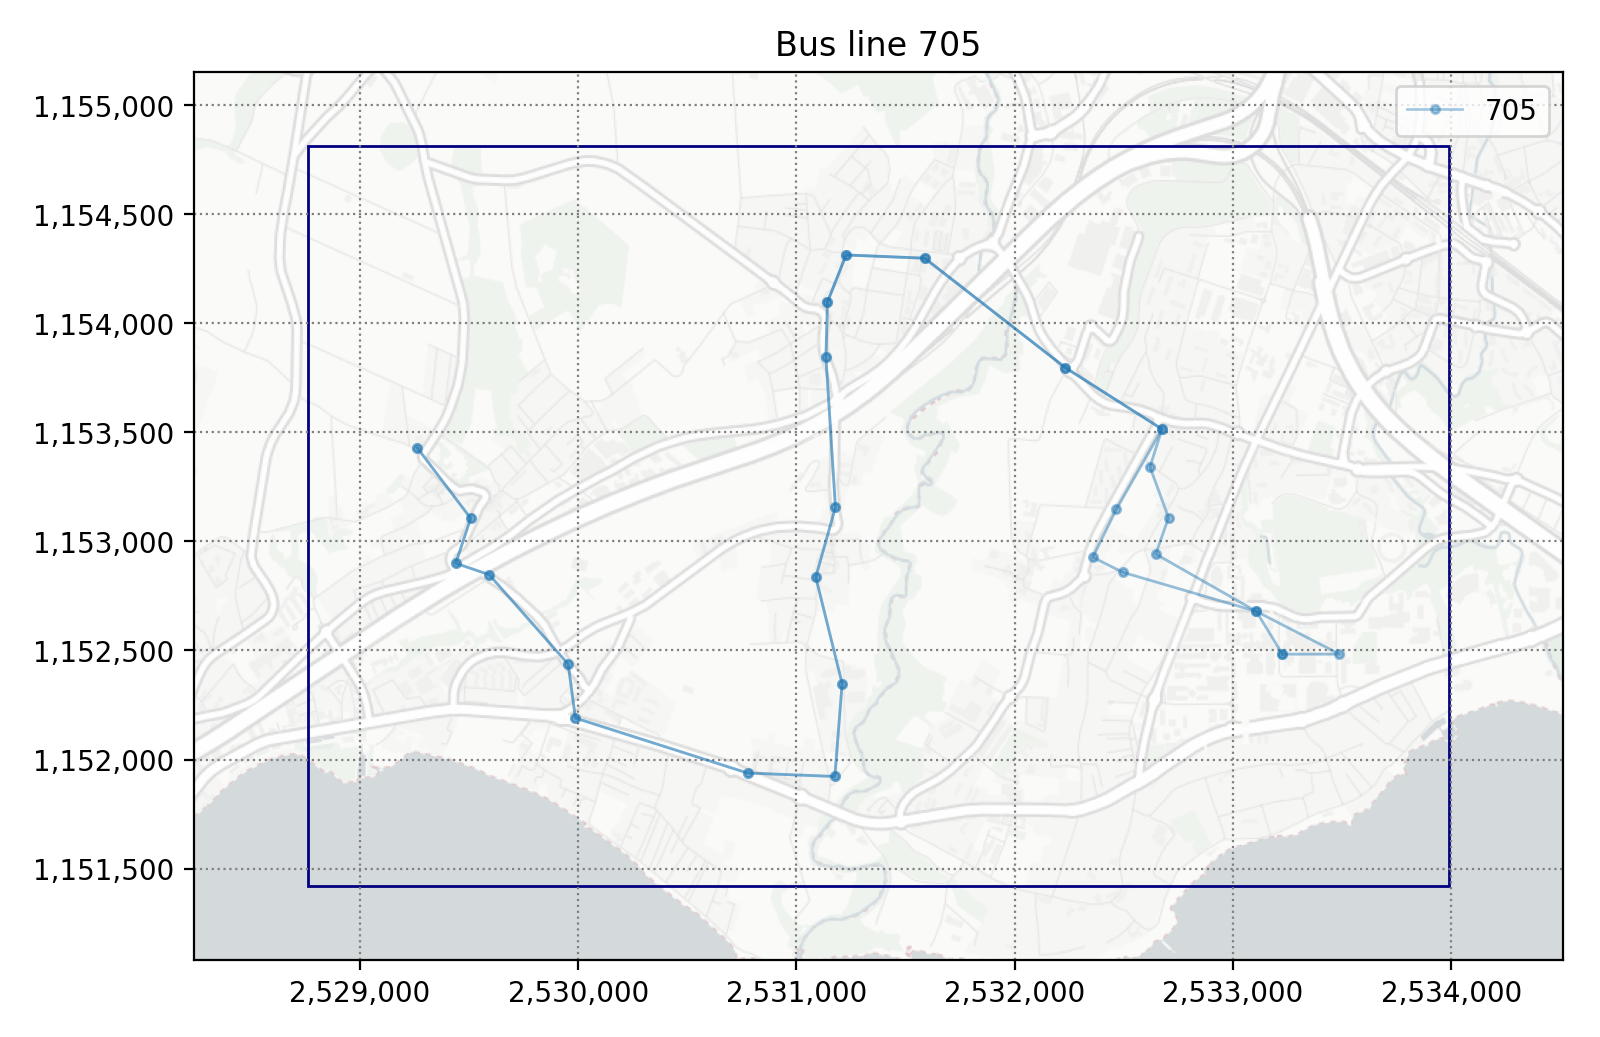
\includegraphics[width=\linewidth]{../fig/l705_area.png}
        \caption{Area considered}
     \end{subfigure}
     \begin{subfigure}{0.8\linewidth}
        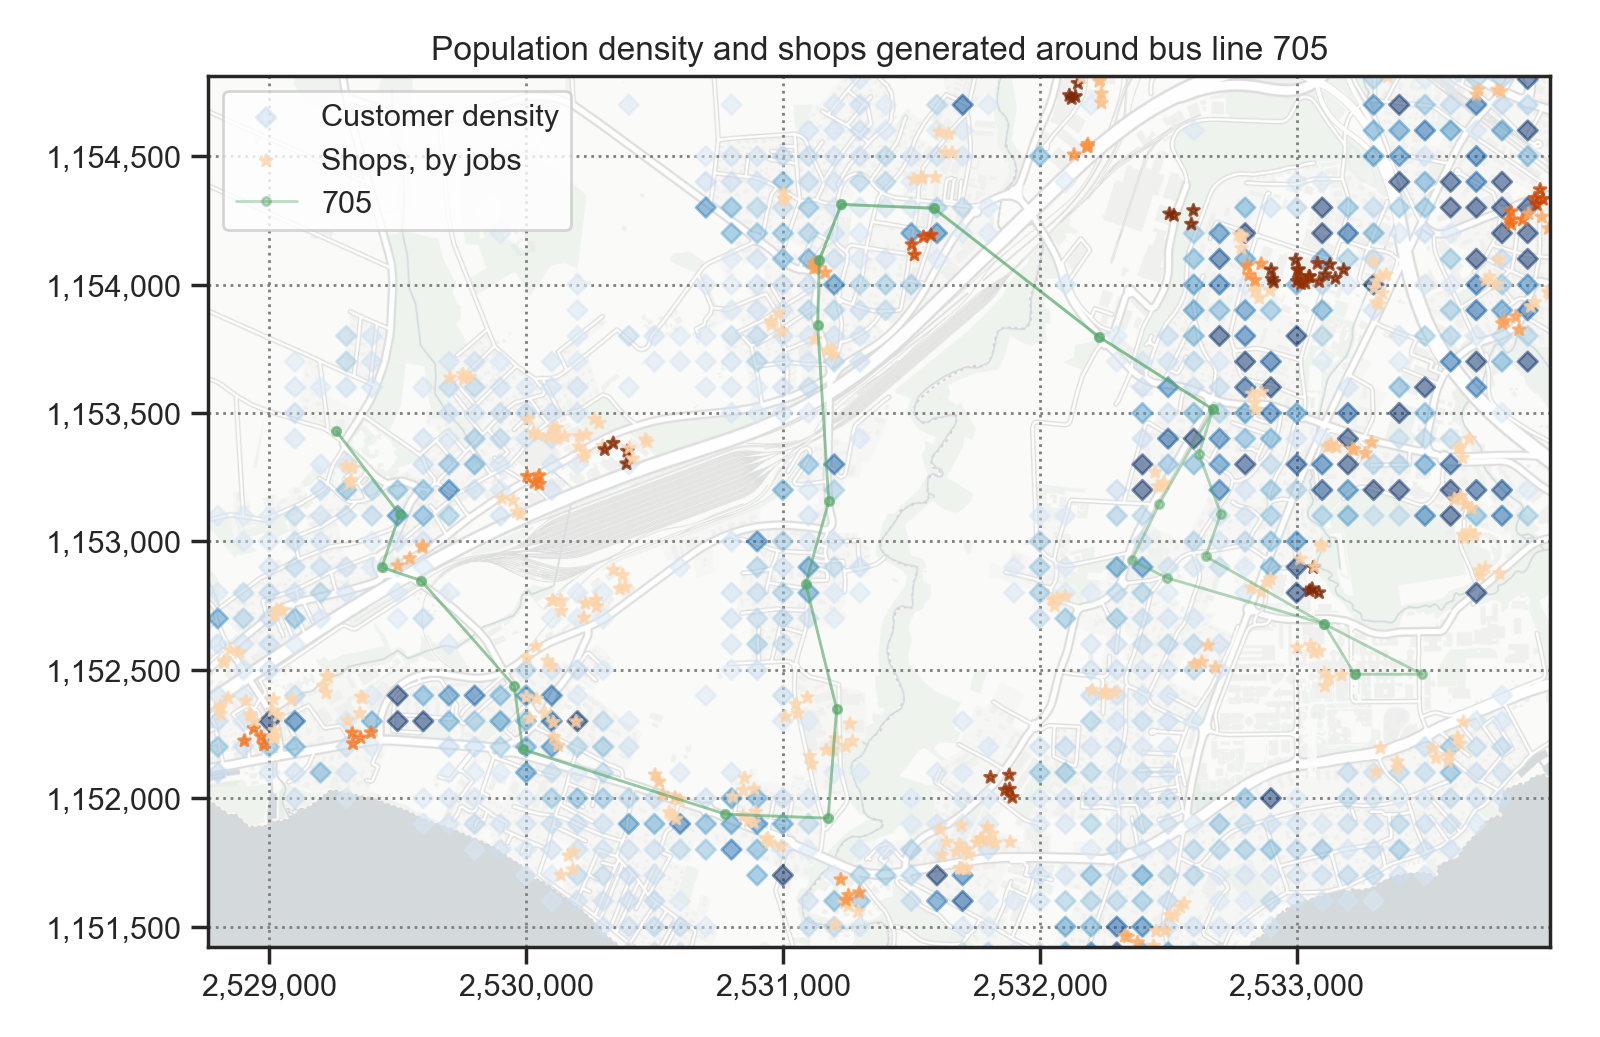
\includegraphics[width=\linewidth]{../fig/l705_densities.png}
        \caption{Population densities and generated shops}
        \label{fig:suburban_densities}
     \end{subfigure}
     \caption{Suburuban case : surroundings of bus line 705}
     \label{fig:suburban_case}
\end{figure}

Looking at the population and shops (Figure \ref{fig:suburban_densities}), we can see the bus line desserves pretty well the population, with the exception of the St Sulpice village in the south and of the Ecublens/Chavannes-près-Renens centers at the north-east, which countain a high density of population and shops.

\subsection{City case : Lausanne agglomeration}

For the third case, we wanted to explore a more complete environment, at a larger scale. We choose for that the Lausanne agglomeration, as depicted in Figure \ref{fig:agglo_case}, as it involves the whole city of Lausanne and surroundings municipalities. In particular, as we can see in the population densities, this area includes the dense city centre, the greater agglomeration with Renens as a second pole, and then outspots, such as the Romanel, Crissier, St Sulpice municipalities. Following population, transport lines radiate from the city and desserve most of the population, altough we could identify a significant zone not well desserved (around coordinates $(2,536,000\text{ , }1,157,000)$), which could be explained that it is desserved by the LEB train and therefore ignored by the bus network. This is an interesting case of some places where the drones would not much benefit from the bus network but the customers could still expect to be served by the delivery system as they are a part of the agglomeration. To account for the greater population, 1000 tasks will be generated.

\begin{figure}
    \centering
    \begin{subfigure}{0.49\linewidth}
       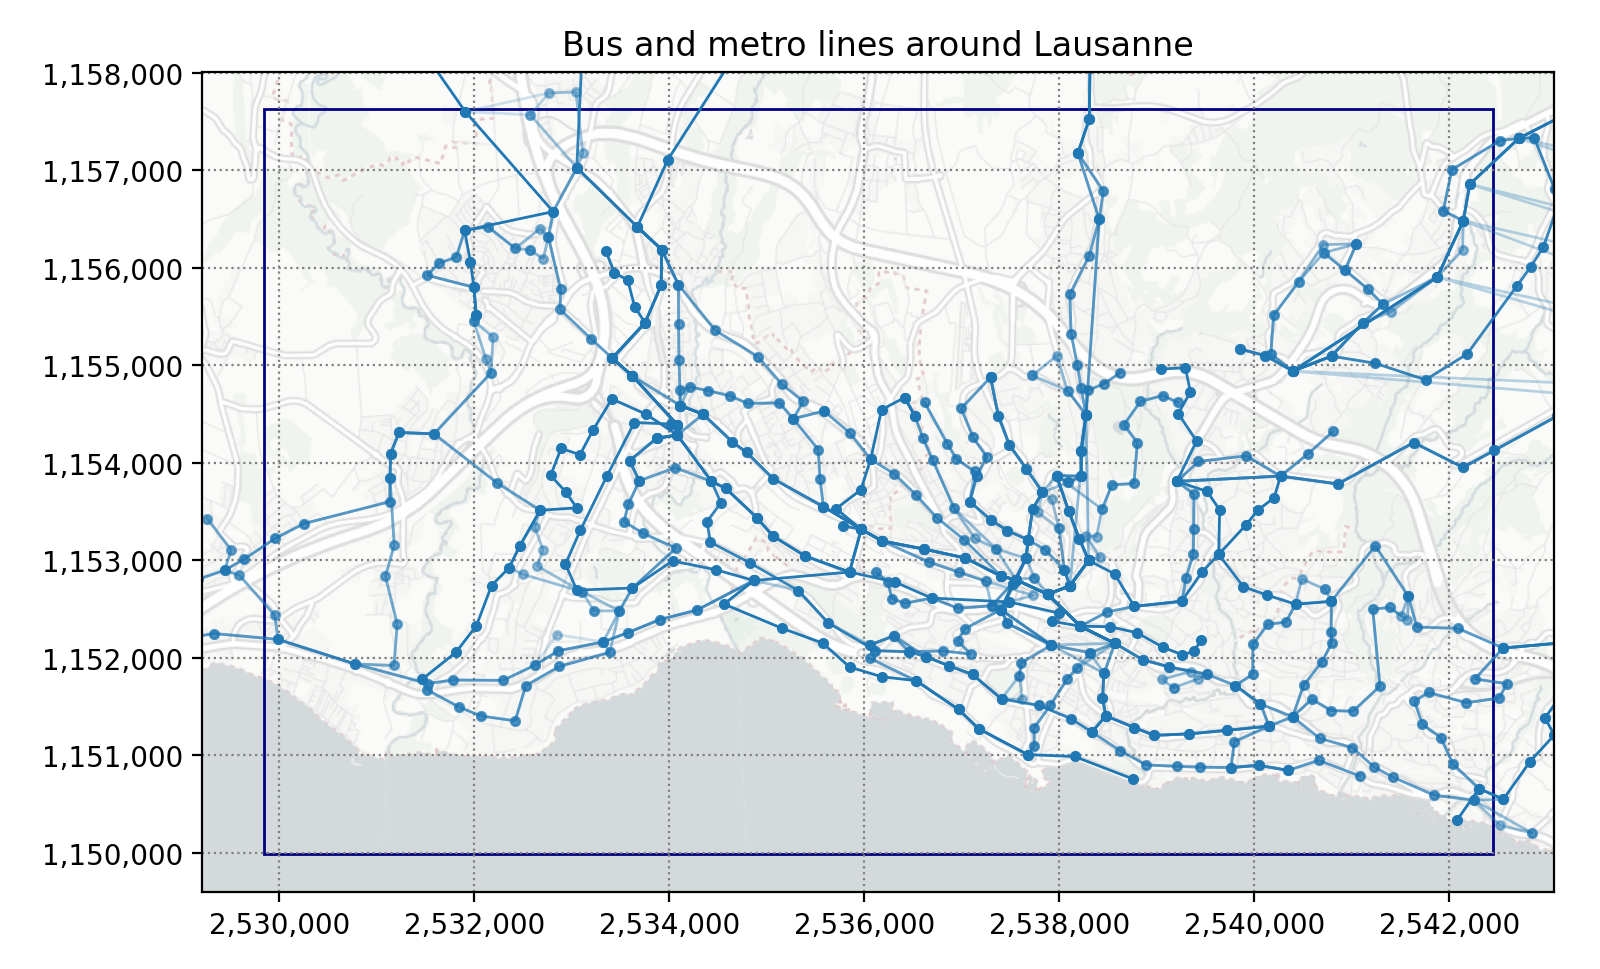
\includegraphics[width=\linewidth]{../fig/laus_bus.png}
       \caption{Area and bus lines considered}
       \label{fig:agglo_area}
    \end{subfigure}
    \begin{subfigure}{0.49\linewidth}
       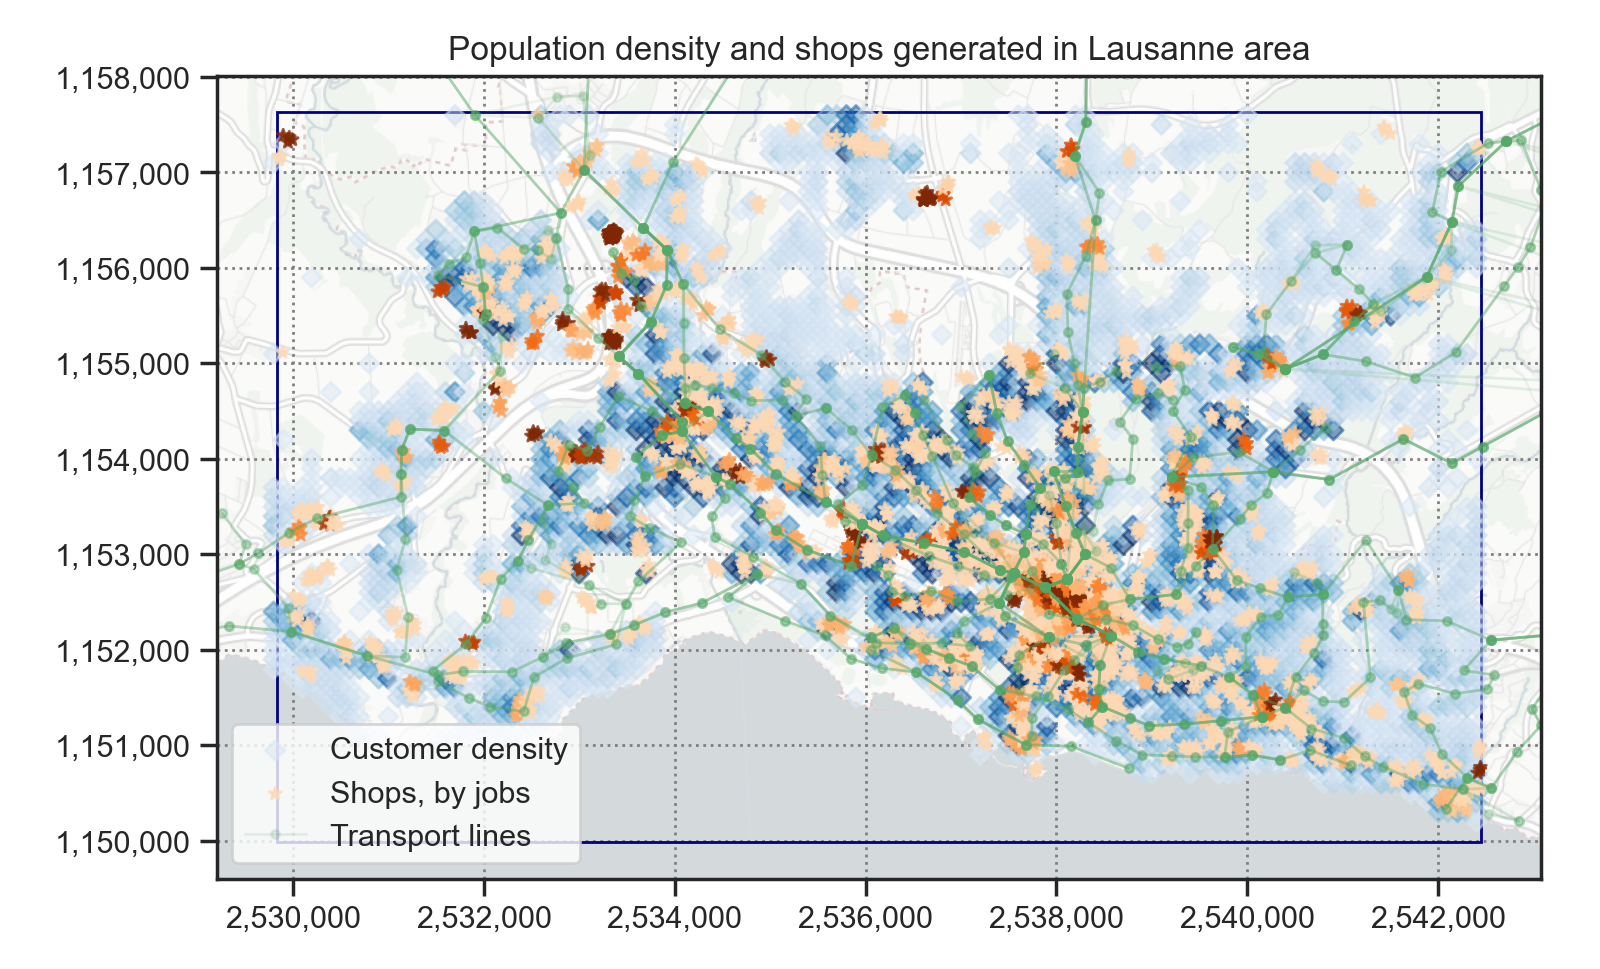
\includegraphics[width=\linewidth]{../fig/laus_density.png}
       \caption{Population densities and generated shops}
       \label{fig:agglo_densities}
    \end{subfigure}
    \caption{City case : Lausanne agglomeration}
    \label{fig:agglo_case}
\end{figure}

\addfigure[agglo_tasks]{laus_tasks1000.png}{City case : Tasks generated}

\subsection{Results}

The drone trajectories with and without using the bus lines are depicted for each case in Figure \ref{fig:results}. For visualisation purposes, we represented on the maps the packages for which the improvement would be negative as not using the bus network and instead going directly to the delivery point, with a black arrow.

\begin{figure}
    \centering
    \begin{subfigure}{\linewidth}
        \centering
        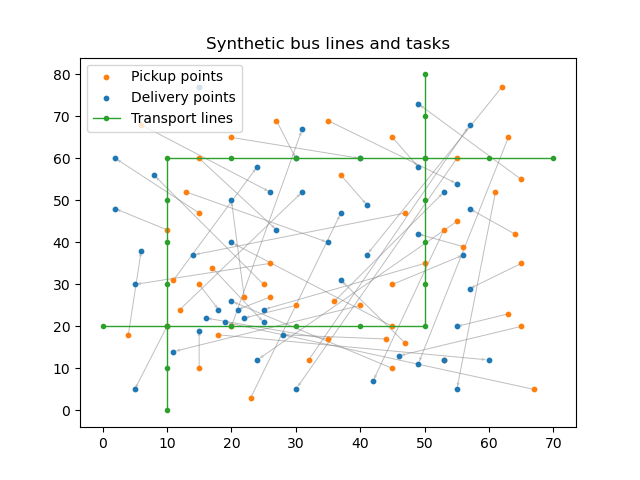
\includegraphics[width=0.49\linewidth]{../fig/synthetic_tasks.png}
        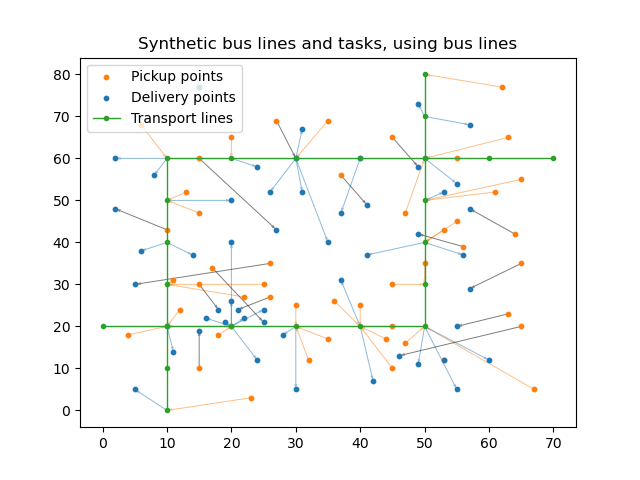
\includegraphics[width=0.49\linewidth]{../fig/synthetic_tasks_bus.png}
        \caption{Baseline case}        
    \end{subfigure}
    \begin{subfigure}{\linewidth}
        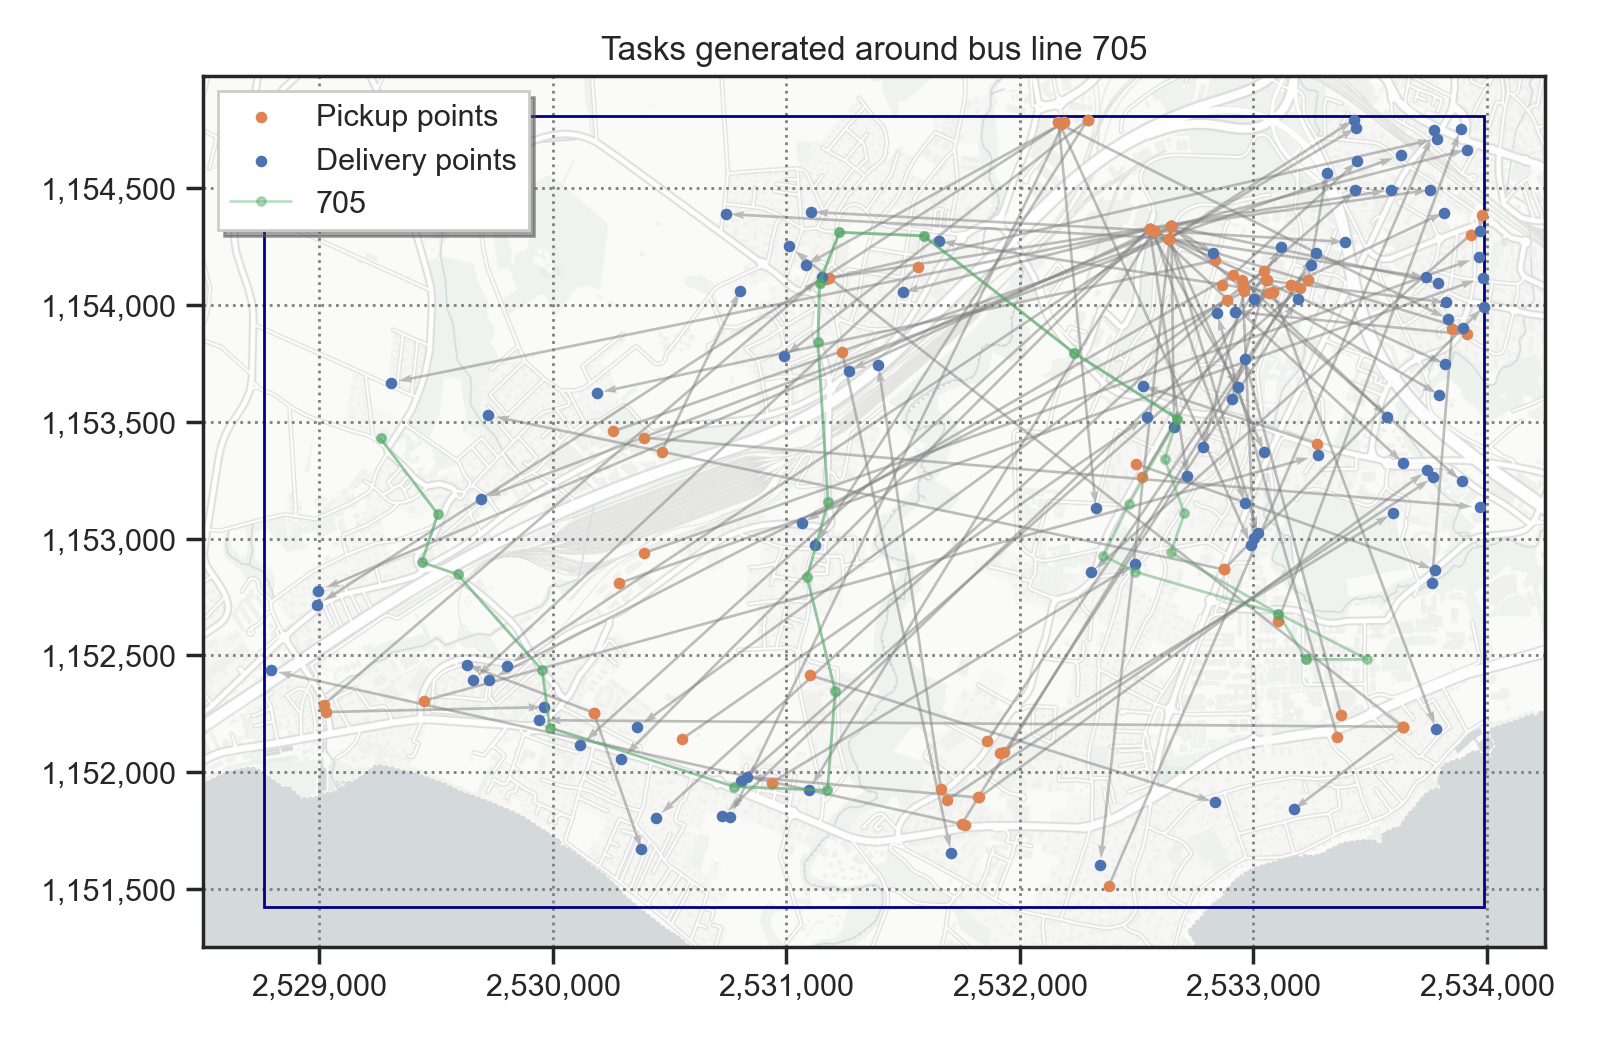
\includegraphics[width=0.49\linewidth]{../fig/l705_tasks.png}
        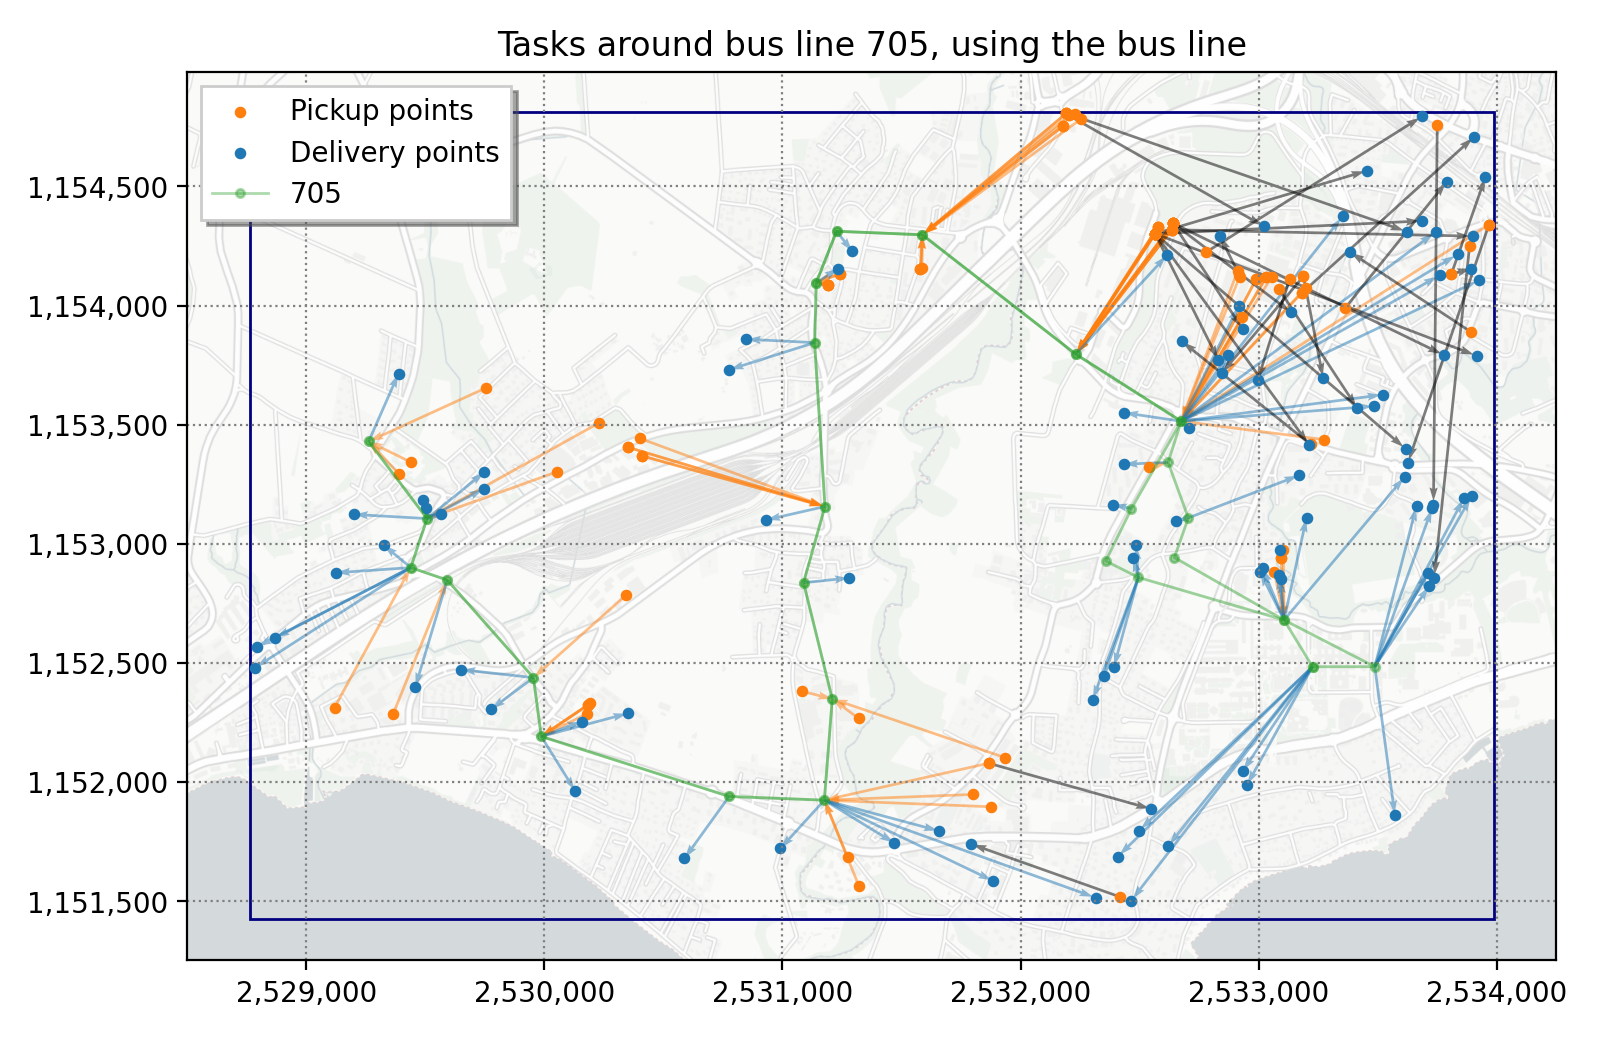
\includegraphics[width=0.49\linewidth]{../fig/l705_tasks_bus.png}
        \caption{Suburban case}        
    \end{subfigure}
    \begin{subfigure}{\linewidth}
        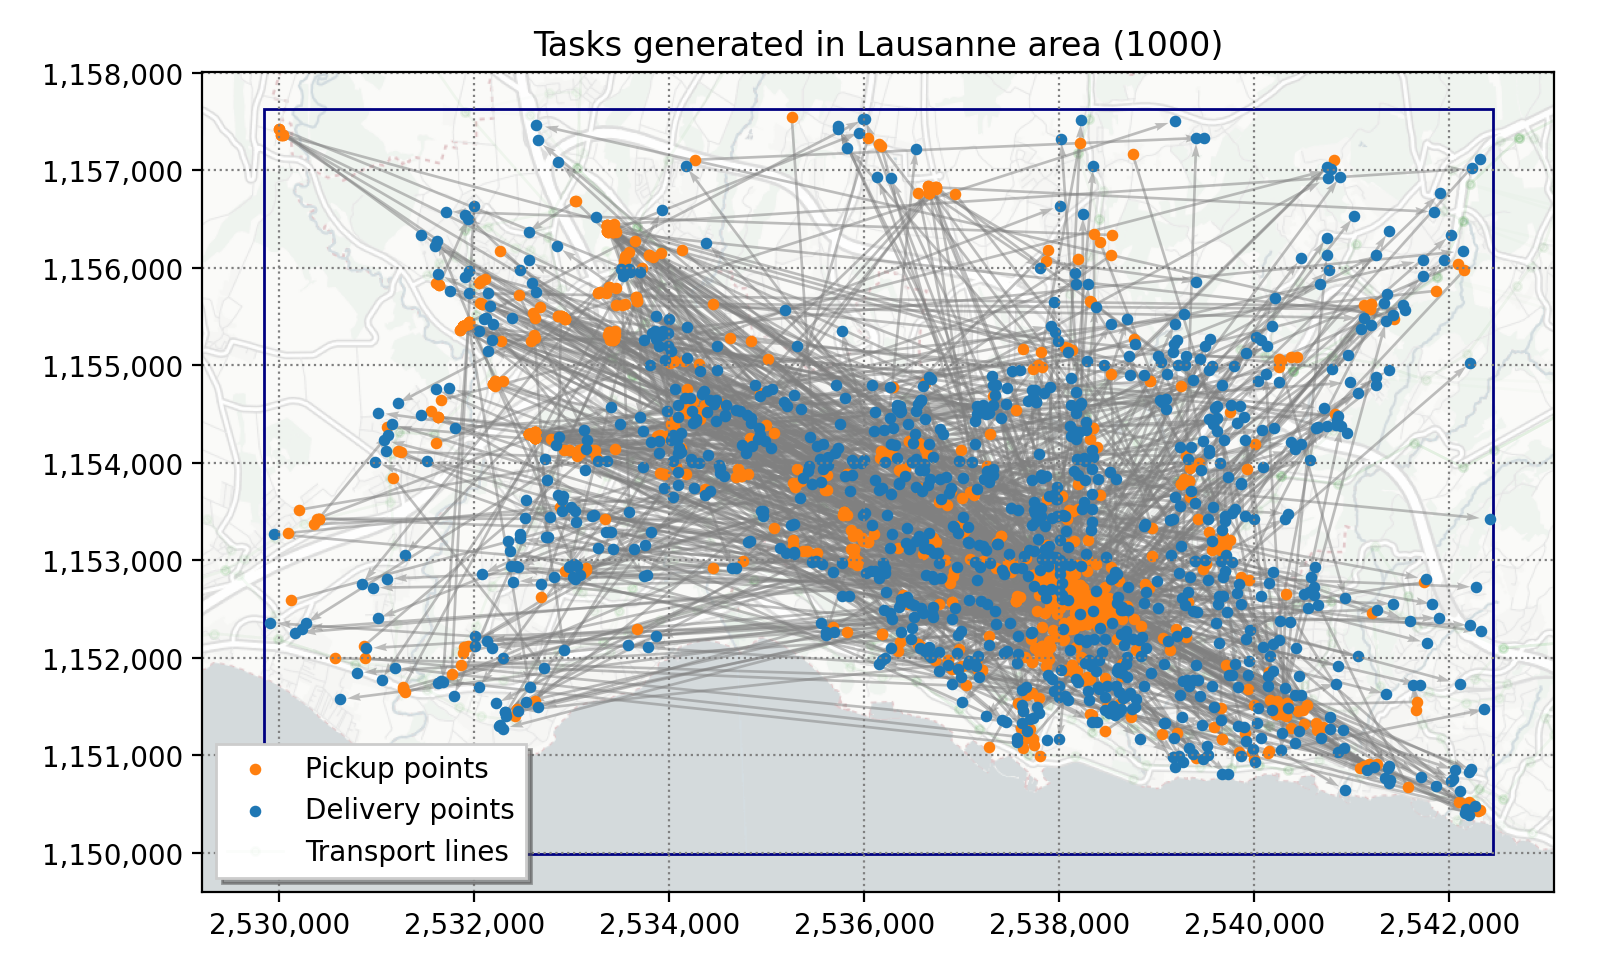
\includegraphics[width=0.49\linewidth]{../fig/laus_tasks1000.png}
        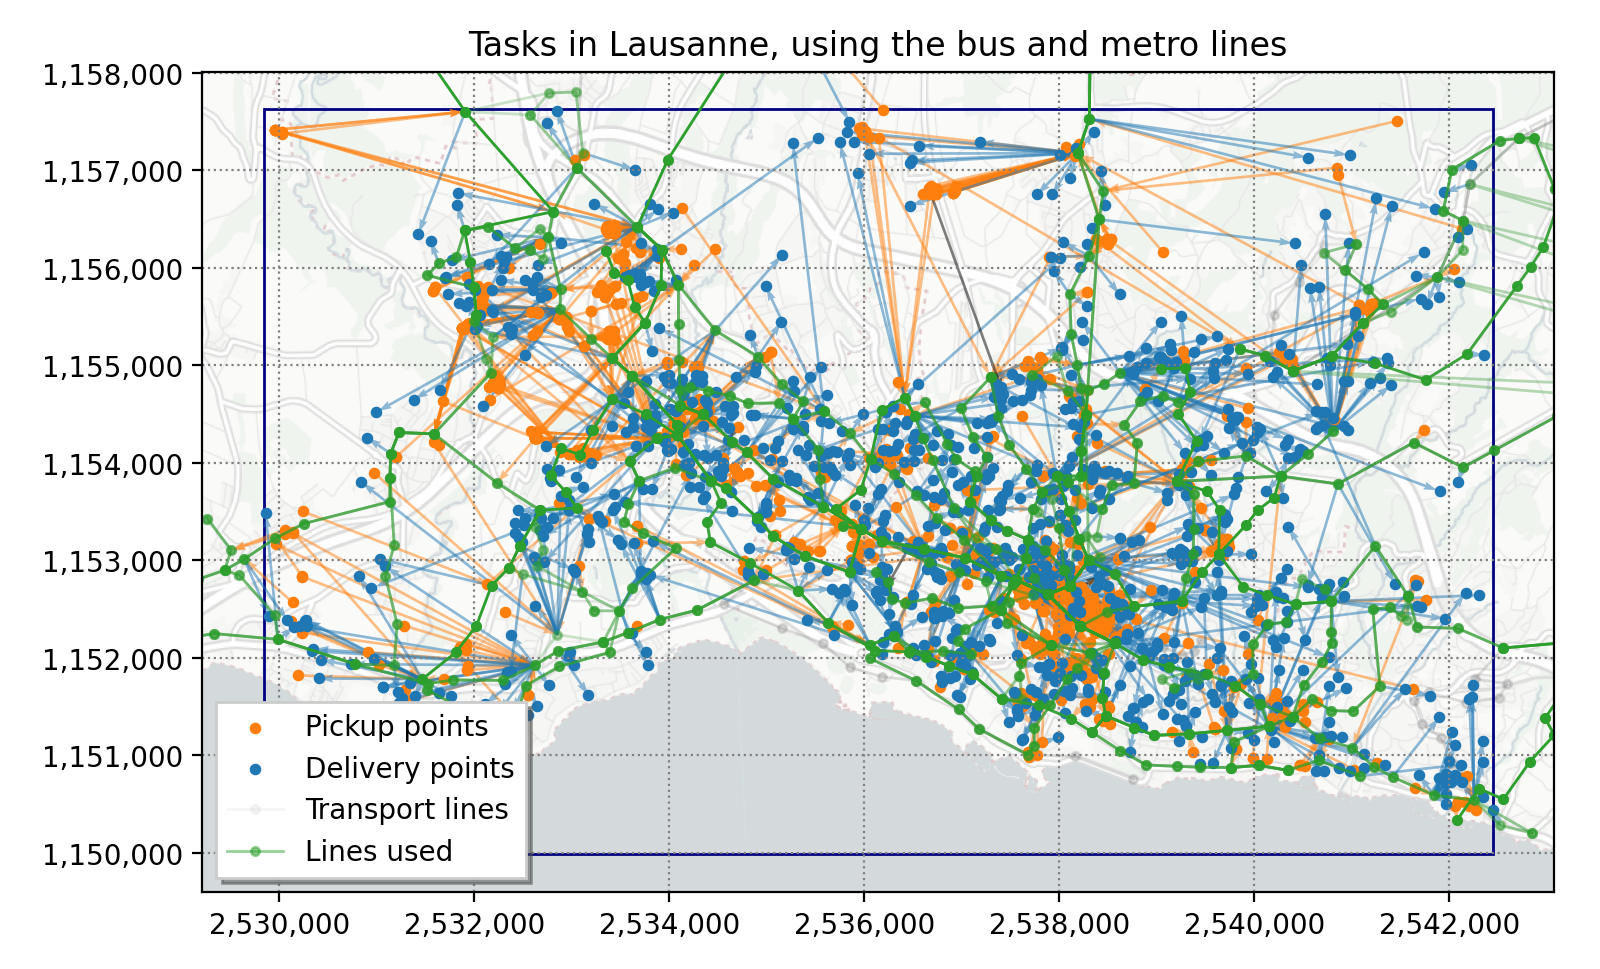
\includegraphics[width=0.49\linewidth]{../fig/laus_tasks1000_bus.png}
        \caption{City agglomeration case}        
    \end{subfigure}
    \caption{Comparison of drone trajectories without using the bus lines (left) and with using the bus lines (right)}
    \label{fig:results}
\end{figure}

%The findings indicate that real data significantly enhances the probability that bus-based deliveries reduce drone travel distances. Moreover, task distributions generated using real data more accurately reflect real-world delivery demands, demonstrating the advantages of this approach over synthetic modeling.